% Tento soubor nahraďte vlastním souborem s obsahem práce.
%=========================================================================
% Autoři: Michal Bidlo, Bohuslav Křena, Jaroslav Dytrych, Petr Veigend a Adam Herout 2019
%-----------------------------------CHAPTER------------------------------------
\chapter{Úvod}
Trend poslední doby byl a stále je neustálé zvětšování obrazovek zařízení i jejich výkonu. Dostali jsme se již do takové fáze, že je tyto zařízení možné využívat obdobně jako klasické počítače a tak je jejich využití pro synchronizaci souborů na snadě.
Vyvíjená aplikace poskytuje systém, který může každý uživatel využít pro svůj účel a svým způsobem. Nejčastěji jet Git využíván programátory pro verzování souborů vyvíjených programů. Rozšíření Git LFS a Git Annex pak pro přidání velkých souborů do těchto repozitářů. Jejich využitím se dosáhne efektivity využití prostoru zařízení a současně plného využití systému Git. Tyto rozšíření lze ale využívat i samostatně. Například pro ukládání videí nebo i jiných velkých souborů na externí úložiště pro pozdější synchronizaci mezi různými zařízeními různých systémů.

Cílem práce je navrhnout, implementovat a otestovat aplikaci určenou pro operační systém Android. Tato aplikace bude uživateli zprostředkovávat Git pro zařízení systému Android formou přívětivého grafického rozhraní. Dále bude implementovat rozšíření \emph{Git LFS} a \emph{Git Annex}. Aplikace je určena zejména vývojářům a jiným pokročilým uživatelům. Je tedy navržena jako maximálně transparentní při zachování prvků jednoduchého ovládání mobilního zařízení.

\newpage
\section {Git}
Git slouží zejména programátorům k verzování jejich práce, popřípadě jejího sdílení s ostatními členy týmu. Nicméně jeho využití je široké a to zejména při využití rozšíření Git LFS nebo Git Annex, která se zaměřují na práci s velkými soubory.

\subsection{Git LFS}
Git Large File Storage (LFS) nahrazuje velké soubory v repozitářích ukazateli. Samotné soubory jsou pak uloženy na vzdáleném serveru. Tento systém tedy slouží k efektivnímu uložení velkých souborů v Git. Jedná se například o video záznamy, zvukové stopy, datasety a jiné velké binární soubory.

\begin{figure}[h!]
    \centering
    \vspace{0.5cm}
    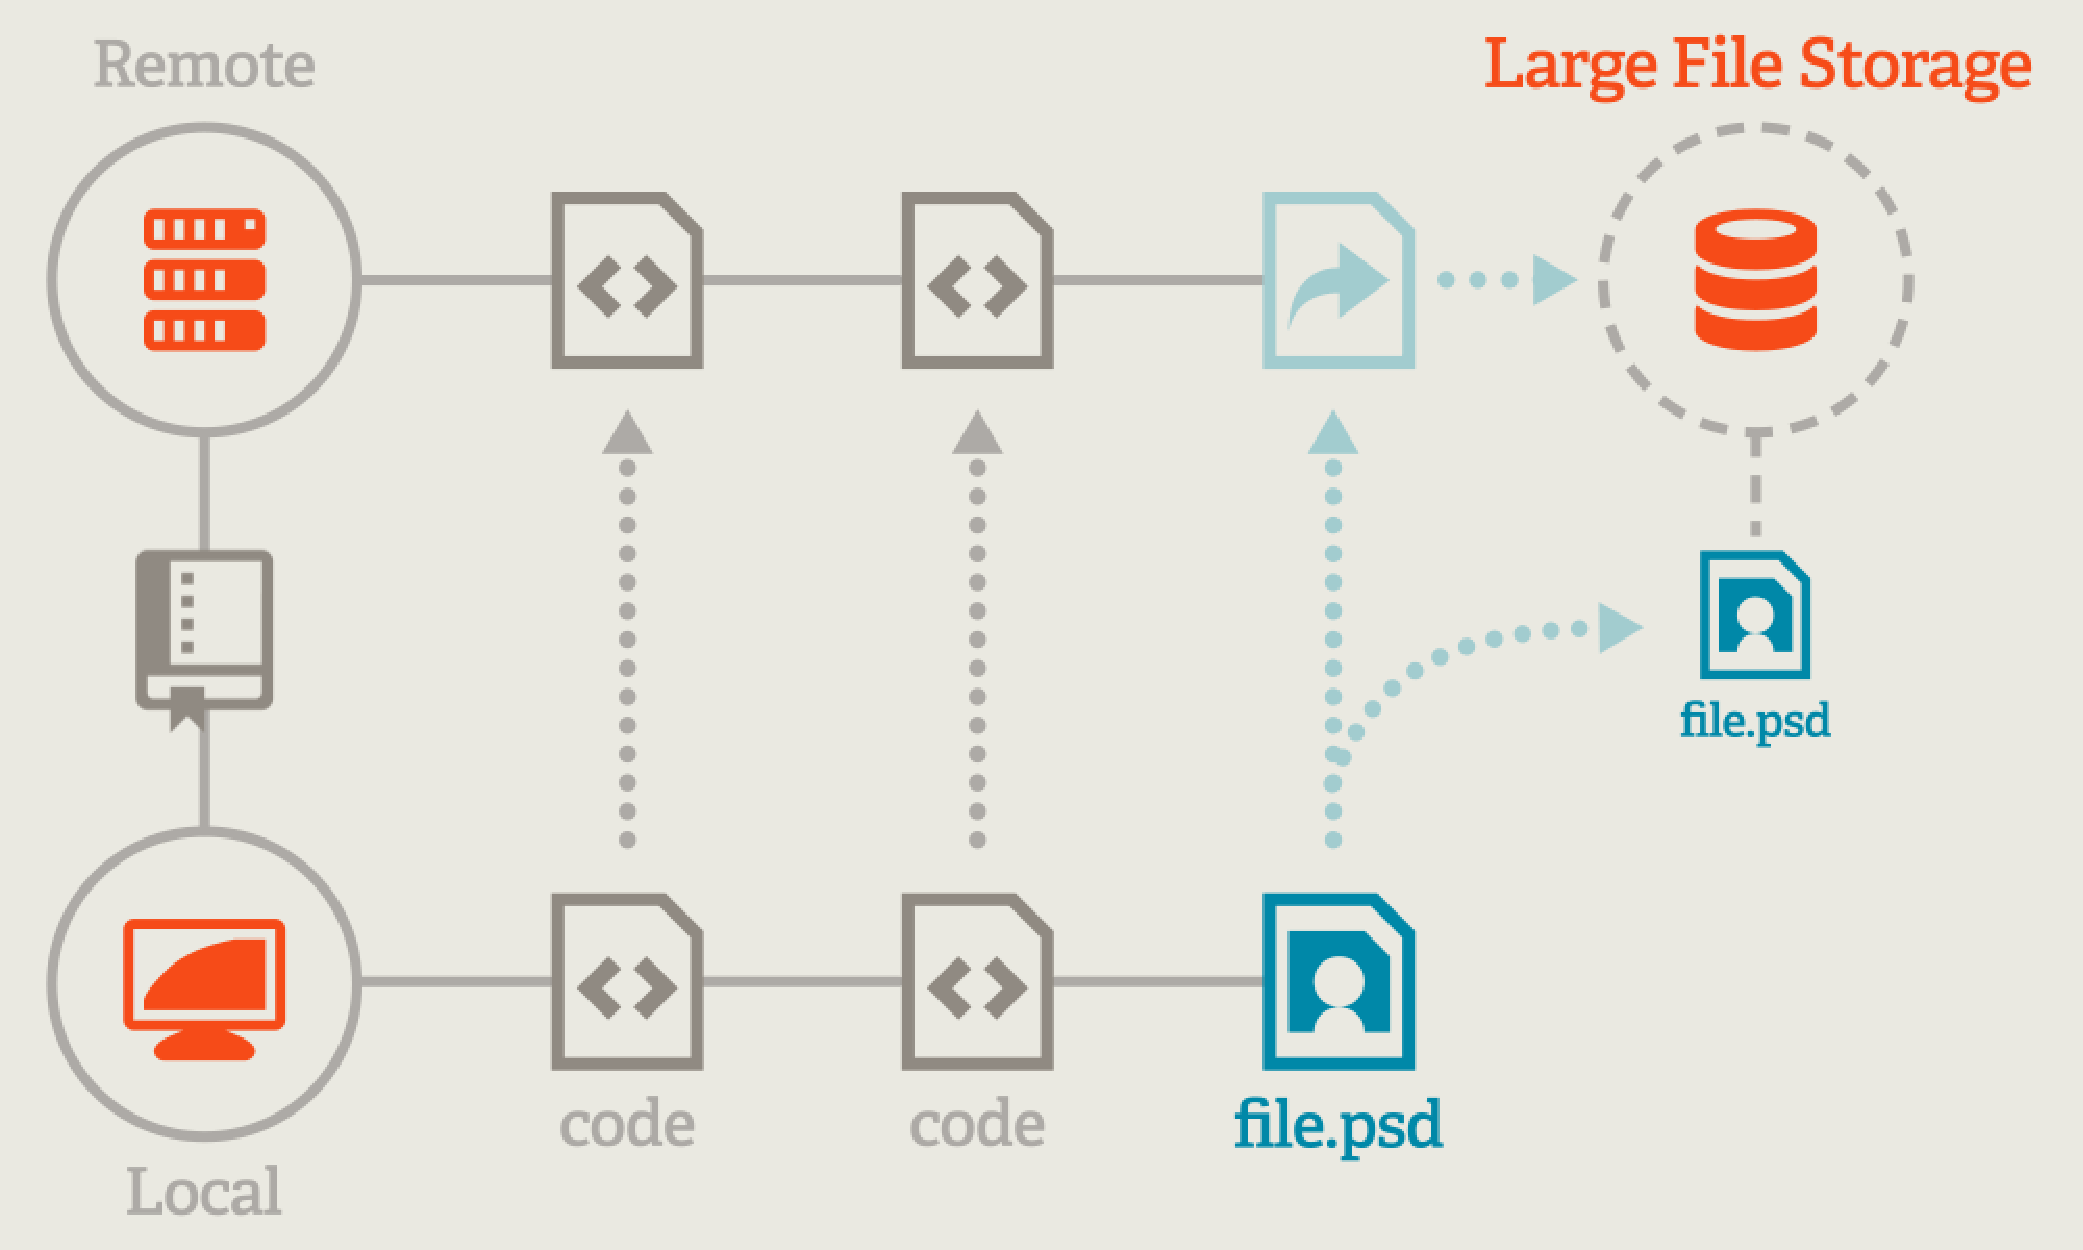
\includegraphics[width=0.75\textwidth,height=0.75\textheight,keepaspectratio]{obrazky-figures/git-lfs.pdf}
    \caption{Architektura Git LFS}
    \label{diagram:git-lfs}
\end{figure}

\subsection{Git Annex}
Git annex slouží k indexaci, synchronizaci a sdílení souborů mezi více úložišti nezávisle na komerční službě nebo centrálním serveru [REF: https://en.wikipedia.org/wiki/Git-annex]. V repozitáři je uložen symbolický odkaz na klíč, který je hash daného souboru. Samotný soubor je pak uložen v adresáři \emph{.git/annex/}. Při změně souboru se mění jen jeho hash a aktualizuje symbolický odkaz. Tímto způsobem je zajištěno šetření místa, jelikož samotný soubor je v repozitáři uložen maximálně jednou.

%-----------------------------------CHAPTER------------------------------------
\chapter{Specifikace řešení}
Hlavním cílem aplikace je nabídnout uživatelům řešení pro verzování a synchronizaci souborů jejich Git repozitářů na zařízení systému Android.

\section{Funkce aplikace}
Aplikace bude mít dvě základní funkce - správa repozitářů a funkce Gitu. Uživatel bude moci spravovat Git repozitáře následujícím způsobem. K přidání nového repozitáře bude mít tři možnosti. Buď může vybrat adresář s daným repozitářem z místních souborů zařízení, inicializovat úplně nový ve zvolené složce nebo klonovat vzdálený. Při otevření repozitáře nad ním může provádět základní funkce Gitu a také některé vybrané funkce již zmíněných rozšíření.

\section{Cílová skupina}
Cílovou skupinou jsou především programátoři nebo i jiní technicky zdatní uživatelé. Ti aplikaci využijí nejčastěji pro prohlížení jejich repozitářů, ale mohou je také jakkoliv měnit a pracovat na nich třeba i z veřejné dopravy. Git annex využijí například při procházení souborů uložených na více fyzických úložištích. Všechny takto sledované soubory budou přehledně zobrazeny v repozitáři a uživatel tak v danou chvíli ani nemusí přemýšlet, kde jsou právě uložené. Jelikož Git annex používá jednoduchý formát Git repozitáře, je navíc garantováno, že tyto data budou v budoucnu dostupná i bez jeho použití.

\section{Průzkum existujících řešení}
Během průzkumu již existující aplikací jsem se zaměřil jak na aplikace operačního systému Android, tak na desktopové operační systémy Linux a Windows.

    \subsection {Android}
    Pro operační systémy Android je trh s řešeními Gitu velice omezený. Existují zde několik málo aplikací s podporou pouze pro čtení repozitáře ale i takové, které zvládají i ostatní základní příkazy Gitu. Jejich popis a mé postřehy z nich se dočtete na následujících řádkách.
    \subsubsection{MGit}
    Za zmínku z nich stojí \emph{MGit}. Bohužel neposkytuje podporu pro \emph{Git LFS} ani \emph{Git Annex}. K implementaci funkcí Gitu využívá knihovnu \emph{JGit}. Ta sice v aktuální verzi podporuje \emph{Git LFS}, ale v té, kterou aplikace využívá ji ještě nemá. K jejím přednostem patří otevřený kód a velice intuitivní ovládání.
    Úvodní obrazovka aplikace se seznam repozitářů. Po kliknutí na některý se zobrazí obrazovka s jeho detaily. Nalezneme zde prohlížeč jeho souborů, log a status repozitáře. Na této obrazovce se také nachází základní ovládací prvek Gitu aplikace. Jím je drawer, který se vysunuje z pravé strany obrazovky. V něm jsou obsaženy všechny poskytované funkce Gitu. Tedy jeho užívání není při porozumění obecného užívání Gitu nijak náročné. Tato aplikace má integrovaný prohlížeč souborů i jejich editování. Ovšem tento editor není dokonalý. Špatně se v něm posouvá kurzor a navíc nemaže konce řádků. Práce s ním je tedy spíše na obtíž. Naštěstí zde autoři přidali i možnost zvolení vlastního editoru z nainstalovaných aplikací.

    \subsubsection{Pocket Git}
    Dále existuje například aplikace \emph{Pocket Git}. Ta je placená a její kód není veřejně přístupný. Využívá integrovaného správce souborů, ale editor již nechává plně na jiných aplikacích. \emph{Pocket Git} má na první pohled přehlednější uživatelské rozhraní. Jednotlivé funkce gitu rozděluje do různých kategorií a vedle souborů přidává ikonku o jeho stavu. Nicméně \emph{Add} a \emph{Commit} jsou natolik integrované do prohlížeče souborů, že jejich správné použití není vůbec intuitivní. Navíc při práci s touto aplikací často narazíte na nejednoznačná chybová hlášení, která neobsahují bližší popis chyby.

    \subsubsection{Termux}
    Pro vývojáře upřednostňující příkazový řádek je možnost instalace aplikace \emph{Termux} a nainstalování Gitu do prostředí jeho terminálu. Tam je i možné doinstalovat rozšíření \emph{Git LFS} a \emph{Git Annex}. \emph{Git LFS} lze doinstalovat přímo jako balíček. \emph{Git Annex} je možné stáhnout z \url{https://git-annex.branchable.com/} a dle návodu uvést do provozu. Obě tato rozšíření lze ovládat z příkazové řádky, přičemž \emph{Git Annex} i přes uživatelské rozhraní. To je implementováno v prohlížeči. Tato webová aplikace je přehledná i pro mobilní zařízení a umožňuje synchronizaci souborů mezi repozitáři různých zařízení.

    \subsection {Desktop}
    Na Linux i Windows existuje mnoho aplikací, které práci s repozitáři zvládají velice dobře. Nicméně prostředí Androidu je od toho desktopového natolik rozdílné, že prostor pro inspiraci je značně omezený.
        \subsubsection{GitKraken}
        Dobré zkušenosti mám například s aplikací \emph{GitKraken}. Ta zobrazuje repozitář přehledně ve stromové struktuře. V ní lze přímo najetím myši na uzel provádět změny. Funkce Gitu má přehledně zobrazené v horním panelu. Navíc jsou zde dobře řešeny konflikty v souborech. Na jedné straně obrazovky vidíte jednu verzi a na druhé straně druhou. Ve spodní části obrazovky se generuje nová verze. Tu vytváříte postupným procházením obou současných verzí a vybíráním vyhovující varianty. \emph{GitKraken} umí pracovat i s \emph{Git LFS}. K ovládání takto sledovaných souborů používá zvláštní vysouvací nabídku s funkcemi \emph{Git LFS}. Ta se v případě práce s repozitářem podporující toto rozšíření zobrazí vedle základních funkcí. Které soubory takto sleduje lze měnit v nastavení repozitáře nebo při přidávání souborů do stage.

        \subsubsection{Ungit}
        Na první pohled dobrým dojmem působí i aplikace \emph{Ungit}. Ta vás při každé akci naviguje krok po kroku a usnadňuje tak používání Gitu pro méně zkušené uživatele. Jedná se o webovou aplikaci založenou na \emph{node.js}. Pro její instalaci je třeba příkazová řádka, pro spuštění pak webový prohlížeč. Její hlavní výhoda je tedy nezávislost na platformě. Její ovládání je rychlé, jelikož aplikace zjednodušuje určité procedury Gitu. Například sama nabízí \emph{Commit} bez nutnosti přidávat soubory do \emph{Stage}. Nicméně aplikace tím zapouzdřuje většinu funkcí. Na základní obrazovce kromě stromu změn repozitáře není další ovládací prvek a aplikace se tak v konečném důsledku jeví až příliš uzavřeně.

        \subsection{Zhodnocení průzkumu}
        Z testování aplikací vyplynulo, že nejjednodušší způsob práce s Gitem je tehdy, když aplikace transparentně zobrazuje funkce Gitu a jejich použití nechá na uživateli. Předejde se tím chybám, jejichž hlášení nejsou vždy dostačující k vyřešení problému. Pokud je funkce dobře zpracována, není třeba vést uživatele krok po kroku. Ovládání se tak urychlí a je stále přehledné.

        Testované aplikace často využívají vlastní textový editor a správce souborů. V obou případech tyto aplikace integrují velice jednoduché verze a jejich použitelnost je tak značně omezená.

        Dalším bodem jsou chybová hlášení. Těm by měla aplikace pokud možno předcházet. Pokud chybě již není vyhnutí, alespoň by měla mít dobrý popis a nebo i návrh jejího řešení.

%-----------------------------------CHAPTER------------------------------------
\chapter{Vývoj aplikací pro systém Android}

%-----------------------------------CHAPTER------------------------------------
\chapter{Návrh aplikace}
    Dle zhodnocení průzkumu a vlastních zkušeností jsem usoudil, že aplikace bude
    \begin{enumerate}
        \item přehledná, ale nebude příliš zapouzdřovat funkce Gitu.
        \item uživatele přehledně informovat o tom co právě dělá, co očekává a jaký je výstup.
        \item využívat externí správce souborů i textový editor.
        \item mít co nejmenší počet za sebou následujících aktivit a tedy i přechodů mezi nimi.
    \end{enumerate}

    \section{Funkce aplikace}
        Git je velice komplexní systém a jeho plná implementace by na zařízeních android byla velice nepřehledná. Proto jsem se rozhodl nejprve implementovat pouze základní funkce Gitu tak, aby aplikace byla funkční a bylo možné další funkce postupně přidávat.

        \subsection{Správa repozitářů}
        Nejdůležitějším ovládacím prvkem aplikace bude seznam sledovaných repozitářů. Repozitář se přidá do tohoto seznamu hned několika způsoby. Prvním je přidání již existujícího repozitáře specifikováním jeho cesty v úložišti zařízení. Druhým je klonování nebo inicializace repozitáře z prostředí aplikace. Tento seznam repozitářů je synchronizován s úložištěm zařízení. Funkce Gitu bude moci uživatel provádět po otevření daného repozitáře.

        \subsection{Funkce Gitu}
        Jelikož žádné aplikace pro Android kromě \emph{Termux} neimplementují rozšíření \emph{Git Annex} a nenalezl jsem knihovnu, která by toto dokázala, bylo rozhodnuto pro funkce Gitu využít zkompilované binární soubory. Mezi tyto funkce patří i funkce jednotlivých rozšíření. Všechny tyto příkazy budou dostupné při otevření repozitáře v bočním výsuvném panelu aplikace. V případě velkého množství takových příkazů budou rozděleny do kategorií, či se zobrazí jen v případě, kdy má jejich užití smysl. Aby uživatel věděl, v jakém stavu se repozitář nachází, budou tyto funkce zobrazovat svůj výstup do textového pole.

    \section{Použité technologie a nástroje}
        Před samotným programováním aplikace bylo třeba udělat průzkum nástrojů, které se při vývoji na zařízení Android používají. Tyto nástroje byly vybrány s důrazem na efektivitu vývoje i náročnost jejich použití. Nejdůležitějším z nich je \emph{Android Studio}[REF], prostředí, ve kterém probíhal vývoj aplikace. Ladění probíhalo většinou na fyzických zařízení z důvodu velké spotřeby RAM Android Emulátorů. Dále vývoj probíhal za užití verzovacího nástroje Git, prostřednictvím aplikace \emph{GitKraken}[REF] na zařízení systému Linux. Kód aplikace byl synchronizován se vzdáleným repozitářem na serveru \emph{GitHub}. Pro dynamické generování instalačních souborů aplikace byl repozitář navíc synchronizován s \emph{GitLab CI/CD}[REF]. Pro vytváření binárních souborů Gitu a Git LFS byl použit \emph{Docker}[REF]. Obraz pro jejich kompilace poskytuje aplikace \emph{Termux packages} [REF: https://github.com/termux/termux-packages].

    \section{Architektura aplikace}

        \subsection{Úvod}
        Aplikace je psána v jazyce \emph{Java}. Dále využívá návrhového vzoru \emph{Model–view–viewmodel} (dále jen MVVM) a \emph{SQLite} databáze. K přístupu k databázi používá \emph{Room Persistence Library} (dále jen Room). Tato knihovna poskytuje abstraktní vrstvu nad databází \emph{SQLite}, zajišťující robustní přístup při plném využití potenciálu tohoto systému řízení báze dat.

        \subsection{Kotlin vs. Java}
        Od 7. května 2019 se \emph{Kotlin} stal preferovaným jazykem vývoje pro Android. Proto jsem od začátku plánoval programovat aplikaci právě v něm. Nicméně během programování aplikace jsem zjistil, že naprostá většina zdrojů na internetu pro řešení problémů pro tuto platformu je psána v Javě. Android studio sice umožňuje zkonvertovat kód do Kotlinu, nicméně ani to není to vždy dokonalé. Užití Kotlinu má tu výhodu, že dovoluje programátorovi vynechat určité části kódu, které jsou nutné pro běh aplikace, ale přímo neřeší daný problém. V angličtině se pro ně vžil výraz boiler-plate code. Ovšem tento kód je přesto třeba vygenerovat, ale o to se již stará Kotlin. To je také jeden z důvodů, proč Kotlin trvá déle zkompilovat. Pokročilým Android developerům jistě přijde rychlejí práce vhod, ale jako začínají programátor na této platformě více ocením transparentnost Javy.

        \subsection{Instalace}
        Jak již bylo zmíněno, aplikace bude pro funkce Gitu využívat binárních souborů. Ty je samozřejmě nutné do prostoru aplikace nějakým způsobem přenést. Z důvodu architektury systému Android není tato operace tak jednoduchá jako například na desktopovém systému Linux. Na výběr bylo z několika možností.

        Z implementačního pohledu nejjednodušší způsob je užití binární knihovny s příponou \emph{.so}. Tuto knihovnu je třeba v rámci struktury aplikace umístit do správného adresáře a systém Android si s její instalací poradí během samotné instalace aplikace. Tato metoda je dobře aplikovatelná v případě, že máte k dispozici staticky linkované binární soubory. Takové soubory v sobě obsahují všechny potřebné závislosti a jejich použití je tak možné samostatně. Ty lze vytvořit křížovou kompilací. Samozřejmě jsem na křížovou kompilaci Gitu nenarazil jako první. Staticky linkovaný Git je možné získat například využitím tohoto repozitáře [REF https://github.com/EXALAB/git-static]. Problém Gitu tkví v tom, že pro jeho funkčnost je třeba více binárních souborů. Git totiž pro každý jeho příkaz používá zvláštní soubor. Ty slouží ke změně chování daného příkazu. Většina z nich jsou dynamické odkazy odkazující na binární soubor programu git. Ale existují zde i takové, které gitu zajišťují určité funkční části. V případě staticky linkovaných binárních souborů všechny tyto soubory musí mít přímo v daném souboru zahrnuté všechny závislosti. A samozřejmě mezi ně patří i samotný git a mnoho dalších knihoven. V součtu je tak velikost takového balíku přes 800MB, což je pro zařízení Android, které má omezenou velikost úložiště, příliš.


        \subsection{Databáze}
        Databáze je využívána pro získání přehledu o repozitářích Gitu, které chce uživatel aplikací sledovat. Každý takový repozitář je reprezentován tabulkou databáze \emph{repo}. Tato tabulka obsahuje absolutní cestu ke složce repozitáře, status repozitáře. Dále případně vzdálené URL, uživatelské jméno a heslo ke vzdálenému repozitáři a další dodatečné informace. Všechny tyto položky je třeba při provádění příkazů Gitu aktualizovat tak, aby stav tabulky v okamžitém časem odpovídal stavu repozitáře.

        \subsection{Návrhový vzor}
        %REF: https://developer.android.com/jetpack/docs/guide
        \emph{Model–view–viewmodel} je v době psaní této práce doporučovaným návrhovým vzorem Android aplikací. K volbě tohoto návrhového vzoru dopomohlo také využití knihovny \emph{Room}. Tato knihovna totiž spoléhá na využití \emph{MVVM} vzoru alespoň pro účely funkčnosti databáze. Je tomu tak proto, že data, která závisí na databázi se ukládají do proměnné datového typu \emph{LiveData}. Hodnotu této proměnné lze sledovat a na jejím základě řídit běh aplikace. Aby byla hodnota této proměnné perzistentní při běhu aplikace, uchovává se její hodnota ve \emph{viewmodelu}. Hlavní takovou proměnnou je v této aplikaci seznam všech Git repozitářů. Ta se nachází ve třídě \emph{RepoRepository}, nicméně její instanciace se provádí pouze v části \emph{view\_model} MVVM.

        \newpage
        \subsection{Balíčky}
        Podle zaměření tříd je aplikace dělena do třech základních balíčků. Jsou jimi \emph{java}, \emph{assets}, a \emph{res}. V balíčku \emph{java} je specifikováno chování aplikace. Balíček \emph{assets} obsahuje soubory nutné pro běh aplikace. V této aplikaci to budou binární spustitelné soubory Gitu. Posledním balíčkem je \emph{res}. Ten obsahuje všechny layouty, ikony a další grafické i textové prvky, které aplikace používá pro grafické rozhraní.

        Následující popis funkčnosti a závislostí balíčků se bude týkat balíčku \emph{java}. Záměrně byl z diagramu vynechán balíček \emph{utilities}. Jeho třídy lze použít kdekoliv v aplikaci a pro budoucí vývoj aplikace jeho zahrnutí nemá opodstatnění.

        \begin{figure}[h]
            \centering
            \vspace{0.5cm}
            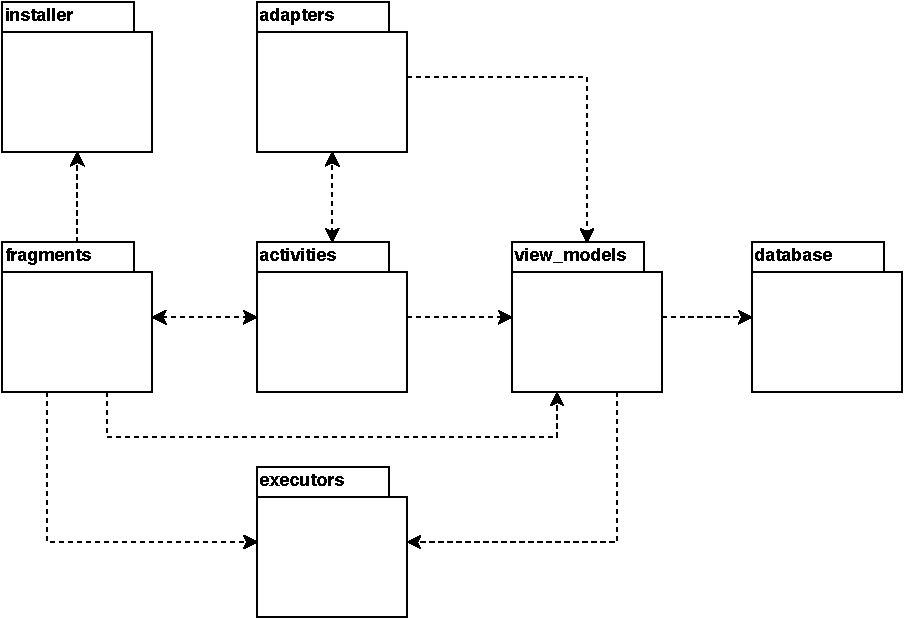
\includegraphics[]{obrazky-figures/drawio/package_diagram.pdf}
            \caption[Diagram závislostí balíčků]{Diagram závislostí balíčků}
            \label{diagram:packages}
        \end{figure}

            \newpage
            \subsubsection{activities}
            Nejdůležitější součást balíčku \emph{Java} je balíček \emph{activities}. Ten aplikaci dělí na obrazovky a o každou z nich se stará jedna třída. Tedy v případě, že aplikace potřebuje určitou obrazovku, je zavolána příslušná aktivita s jejím chováním. Všechny aktivity aplikace rozšiřují základní aktivitu \emph{BasicAbstractActivity}. Ta implementuje společné prvky rozhraní aktivit. Například získávání oprávnění, zobrazení různých oznámení a dialogů.

            \subsubsection{adapters}
            Tento balíček obsahuje třídy, které slouží k zobrazení položek stejného typu. Tato aplikace je využívá k zobrazení seznamu repozitářů základní obrazovky a funkcí Gitu v bočním výsuvném panelu.  

            \subsubsection{database}
            Tento balíček obsahuje balíček \emph{model}, ve kterém se nachází třída Repo. Ta implementuje tabulku databáze uchovávající všechny potřebné informace o repozitáři. Instance databáze se uchovává ve třídě \emph{RepoDatabase}. K přístupu k ní se využívá třída \emph{RepoDao}. Tato třída obsahuje metody volající \emph{SQLite} dotazy databáze. Aplikaci je databáze zprostředkována třídou \emph{RepoRepository}, která odpovídá \emph{Repository} modelu MVVM.

            \subsubsection{fragments}
            Fragmenty, třídy které dynamicky rozšiřují nebo mění obsah aktivity. Aplikace používá fragmenty například k instalaci a nastavení. Každá aktivita může obsahovat několik fragmentů, které samostatně řeší určitou část aktivity.

            \subsubsection{installer}
            O instalaci binárních souborů se stará třída \emph{AssetInstaller} v balíčku \emph{installer}. Ta při prvním spuštění aplikace zkopíruje potřebné soubory ze složky \emph{assets} do interní paměti zařízení. Systém Android podporuje symbolické odkazy. Ovšem při kopírování souboru symbolického odkazu dochází ke kopírování souboru, na který odkaz odkazuje, nikoliv samotného odkazu. Proto je nutné tyto odkazy vytvářet během instalace zvlášť.

            \subsubsection{executors}
            Základní funkce Gitu i jeho rozšíření \emph{Git Annex} a \emph{Git LFS}, jsou implementovány v balíčku \emph{executors}. Tyto třídy rozšiřují základní třídu \emph{AbstractExecutor} využívající \emph{ProcessBuilder}. Ta spustí binární soubor, který vykoná danou funkci Gitu na zařízení.

            \subsubsection{utilities}
            Jedná se o statické metody a proměnné, které jsou použitelné kdekoliv v aplikaci. 

            \subsubsection{view\_models}
            Třídy obsahující perzistentní data a implementující logiku nad nimi. Tento balíček odpovídá části \emph{ViewModel} MVVM. Tento balíček tak poskytuje aplikaci metody zajišťující její funkčnost. Komunikace mezi ViewModely a aktivitami je zajištěna pomocí databindingu, observerů a veřejných metod, které poskytují.

        \subsection{Obrazovky Aplikace}
        Aplikace bude rozdělena podle obrazovek do aktivit. Tyto aktivity dále mohou obsahovat různé fragmenty. Ke každé aktivitě, která poskytuje určitou obrazovku je připojen její ViewModel. Ten jí poskytuje data a funkcionalitu. Vzhled obrazovky je dán jejím layoutem.

    \section{Manipulace se soubory}
    Průzkumník souborů je možné implementovat různými způsoby s různým stupněm jeho komplexnosti. Proto je pro prohlížení souborů repozitářů využíváno externího aplikace. Uživateli je tak ponechána volnost při jeho volbě a předejde se tak hledání kompromisů pro jeho implementaci.

    Jelikož úprava souborů probíhá za použití průzkumníku souborů, je logické, že textový editor je rovněž využit z externích aplikací.

    \section{Grafické uživatelské rozhraní}
    Grafické rozhraní se nejvíce inspiruje aplikací \emph{MGit} a přidává prvky vzniklé z požadavků na aplikaci. Především se jedná o zpracování rozlišení repozitářů, které podporují jedno z rozšíření. V případě, že repozitář bude podporovat \emph{Git LFS} přidají se dané funkce do draweru k ostatním funkcím Gitu. Dále se do nastavení repozitáře \emph{Edit repository} přidá možnost změnit sledované soubory tímto rozšířením podle jejich přípony.

%-----------------------------------CHAPTER------------------------------------
\chapter{Implementace}

%-----------------------------------CHAPTER------------------------------------
\chapter{Testování}
%-----------------------------------CHAPTER------------------------------------
\chapter{Závěr}